

\documentclass{article}
\usepackage[utf8]{inputenc}
\usepackage{authblk}
\usepackage{setspace}
\usepackage[margin=0.81in]{geometry}
\usepackage{graphicx}
\graphicspath{ {./figures/} }
\usepackage{subcaption}
\usepackage{amsmath}
%\usepackage{lineno}
\usepackage{hyperref}
\usepackage{indentfirst}
\usepackage{cellspace}
\setlength\cellspacetoplimit{8pt}
\setlength\cellspacebottomlimit{8pt}


\usepackage[toc,title]{appendix}



\usepackage[style=authoryear, sorting=nty, backend=biber]{biblatex}
\addbibresource{bib.bib} % Your .bib file


\title{\textbf{From Optical to X-rays: Probing Environmental Interaction and Electron Acceleration in Gamma-Ray Bursts}}


\author[]{Olivia Nippe-Jeakins, Alexander van der Horst}



\affil[]{\textit{Department of Physics, The George Washington University, Washington, D.C., USA}}


\date{\today}


\onehalfspacing

\begin{document}

\maketitle



\begin{abstract}
The afterglows of gamma-ray burst (GRBs) provide a powerful probe of relativistic jet physics, particle acceleration, and the role of the surrounding environment in shaping their observed emission. In this work, I investigate both environmental effects and intrinsic spectral properties of GRB jets using multiwavelength observations of GRB afterglows. First, I examine the optical darkness of a sample of TeV-detected GRBs to test whether extreme high-energy emission is linked to enhanced circumburst extinction. By computing the broadband spectral index $\beta_{ox}$ from temporally matched optical and X-ray data, I find that TeV GRBs are not systematically more optically obscured than the general long GRB population, suggesting that a particularly dense environment is not the dominant factor driving their energetics. Second, I explore how assumptions in afterglow spectral modeling affect the interpretation of observed emission. Using both sharp and smoothly broken power-law models, I analyze the dependence of optical and X-ray spectral indices on the location of the cooling break frequency, $\nu_c$, showing that smoothly broken spectra produce a continuous evolution in spectral slopes, while sharp-break models introduce unphysical discontinuities. These results demonstrate that much of the observed diversity in GRB spectral indices can be explained by variations in $\nu_c$ rather than requiring significant intrinsic variation in the electron energy distribution index, $p$, which theory predicts is a single fundamental, universal value. 
\end{abstract}



\section{Introduction}


The universe is host to a variety of relativistic, jet-like sources that launch beams of particles at speeds close to the speed of light. Such systems span a range of astrophysical contexts, from active galactic nuclei powered by supermassive black holes to supernova remnants \parencite{white_pap}. Despite the diversity of these sources, they all raise a common set of fundamental questions in high-energy astrophysics: how are particles accelerated to such extreme energies, and how do interactions with the surrounding environment impact observations of these sources?

The physical conditions within relativistic jets cannot be recreated experimentally on Earth as the magnetic field strengths, particle densities, and energies far exceed anything achievable in terrestrial accelerators. As a result, observational astrophysics serves as our primary window into these extreme systems. By studying the light emitted from these sources across the electromagnetic spectrum, spanning radio waves to gamma-rays, we can infer the physical processes that govern our observations of these systems. Interpreting these observations, however, requires careful modeling and an understanding of how both the underlying physics and environmental conditions influence what we detect. 

One astrophysical object of interest for studying relativistic jets are gamma-ray bursts (GRBs). GRBs are the most luminous, explosive events in the universe, briefly outshining entire galaxies \parencite{GRBs_science}. They are widely thought to be produced by either the collapse of massive stars (classified as long GRBs) or by the merger of compact objects like neutron stars (classified as short GRBs). In both cases, a newly formed central engine launches a pair of ultra-relativistic jets as shown in Fig.~\ref{fig:progenitors} \parencite{kouv_1993, fireball}. When one of these jets is pointed toward Earth, we detect a GRB.

Observationally, GRBs consist of two main phases. The first, known as the prompt emission, is a short-lived burst of high-energy gamma-rays that originate from internal shocks within the GRB jet. This is followed by the afterglow, which occurs as the jet collides with the surrounding medium, shocking and accelerating circumburst particles that then emit radiation across a broad range of wavelengths \parencite{fireball, afterglow, inv_Compton}. The afterglow phase is particularly valuable for probing the physics of relativistic jets, because it evolves more slowly and can be observed in detail from radio to gamma-ray energies \parencite{jets_in_GRBs}. 

A particularly intriguing subset of GRBs are those that emit very high-energy gamma-rays, extending into the tera-electronvolt (TeV) range. These TeV GRBs represent the most extreme end of the GRB population, yet the source of their energetics remains uncertain. One proposed explanation is that their environments play a key role, either by influencing how efficiently particles are accelerated or by altering how radiation escapes the system \parencite{VHEGRBs}. When GRB jets interact with the surrounding medium, they produce shocks that accelerate the circumburst material. These accelerated charged particles then produce high-energy photons that we detect here on Earth \parencite{high-energy}. Determining whether environmental interactions are responsible for the energetics of these TeV GRBs is therefore an important step toward understanding their underlying physics. 

\begin{figure}[t]
    \centering
    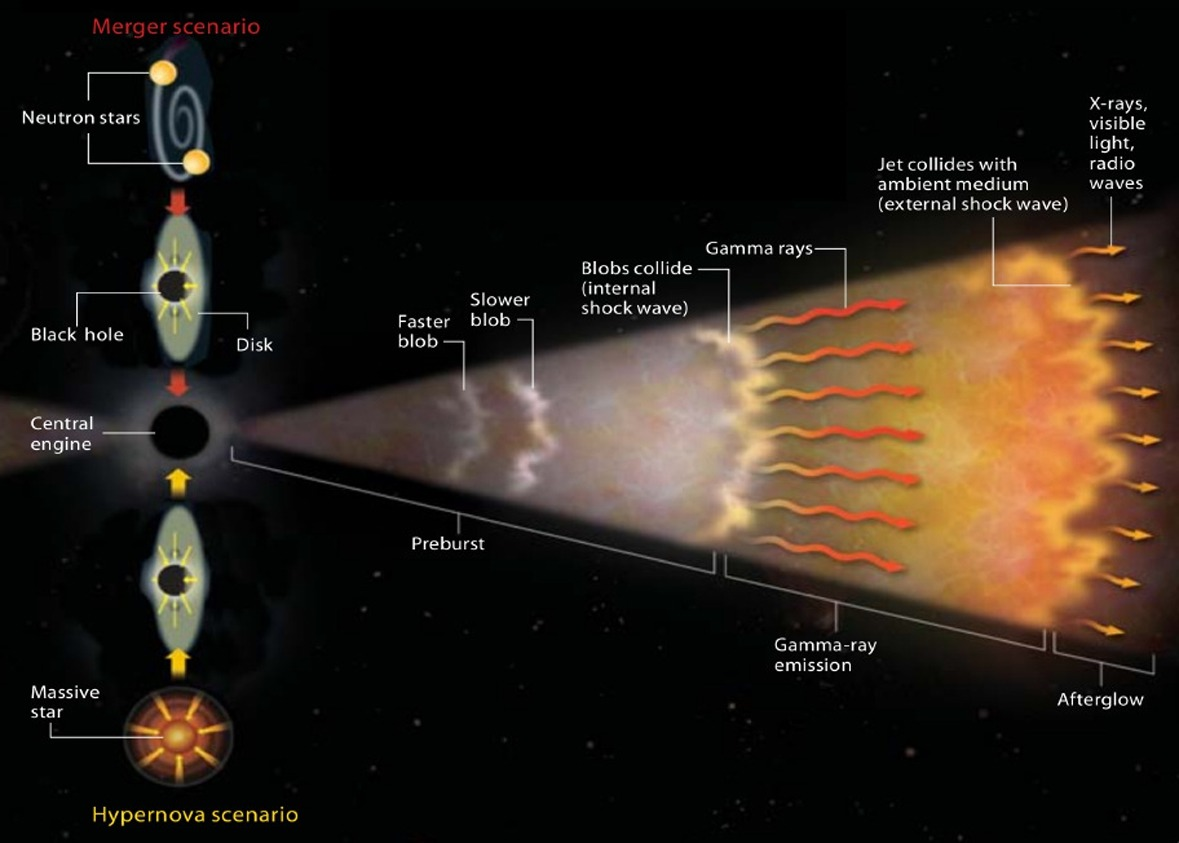
\includegraphics[width=0.95\textwidth]{figures/grb_progenitors.jpg}
    \caption{\centering{Illustration of the two progenitor scenarios of GRBs and their theorized jet structure 
    \\ (from \parencite{sci_am}, credit Juan Velasco)}}
    \label{fig:progenitors}
\end{figure}

The objective of the first part of this study is to investigate this hypothesis by analyzing the optical darkness of all six TeV GRBs that have been observed thus far. Optical darkness is defined by the ratio of optical to X-ray fluxes and serves as a diagnostic of environmental absorption \parencite{jakob, opt_dark}. GRBs that are unusually faint in the optical regime relative to their X-ray emission are classified as “dark bursts,” often interpreted as being embedded in dust-rich or optically thick environments which absorb lower energy optical photons but are transparent to higher energy X-ray photons. This work compares the optical darkness of these TeV GRBs to the broader long GRB population to determine whether TeV GRBs occur in uniquely obscured environments that enable them to produce their characteristic high-energy radiation.

The second portion of this study focuses on the physics of particle acceleration and radiation in GRB jets by examining afterglow spectra across optical and X-ray wavelengths for a large sample of bursts (pulled primarily from the GRB catalogue created by \cite{grb_sample}). Standard analytical models approximate these spectra using sharp spectral breaks at characteristic frequencies, such as the peak flux frequency, $\nu_m$, and the electron cooling break frequency, $\nu_c$. This is not a physical representation as, in reality, these transitions should be smooth as a function of frequency and evolve gradually over time \parencite{breaks}. Another challenge of modeling GRB afterglow spectra is accurately locating these characteristic break frequencies. Misidentifying the locations of these breaks can lead to incorrect inferences about fundamental parameters, including the electron energy distribution index, $p$, which encodes information on the behavior of accelerated electrons. My analysis aims to address the limitations of current GRB afterglow spectral models and offers a new, more physical method of representing GRB radiation and jet dynamics.

By analyzing multiwavelength spectral indices and improving the modeling of spectral breaks, this work aims to constrain the impact of environmental interactions and the process of particle acceleration in GRB jets. Together, these projects address two central questions in high-energy astrophysics: how extremely energetic radiation is produced and how environments shape the signals we detect from the most explosive events in the universe.



\section{Methodology}

An essential component of this study is the use of data from the Neil Gehrels Swift Observatory (hereafter referred to as Swift), a space-based observatory launched in 2004. Swift was specifically designed by NASA to study GRBs, coupling rapid detection with multiwavelength follow-up observations. Its instrumentation includes the Burst Alert Telescope (BAT), which operates in the 15--150 keV range and identifies GRBs in real time by detecting sudden spikes in gamma-ray flux. Once a burst is identified, Swift autonomously slews, or points, to the source location within a matter of seconds. This enables follow-up observations with the onboard X-Ray Telescope (XRT) and Ultraviolet/Optical Telescope (UVOT). The UVOT is sensitive in the 1.9--7.3 eV range while the XRT detects within the 0.3--10 keV range, providing detailed temporal and spectral measurements of the GRB afterglow. These measurements are critical for determining spectral indices and characterizing broadband emission properties \parencite{swift}.

Historically, GRB afterglow observations have been restricted by delayed localization, limited temporal sampling, and incomplete spectral coverage. Prior to the Swift era, X-ray and optical follow-up often began hours after the prompt emission, restricting insight into early time evolution and spectral transitions \parencite{oates}. The rapid-response capability of Swift, combined with ground-based optical observatories and the development of high-energy detectors, has enabled densely sampled, multiwavelength light curves spanning from minutes to weeks post-burst. This expanded coverage in both time and frequency makes it possible to track the evolution of spectral breaks, constrain broadband spectral slopes, and test afterglow models with significantly improved precision \parencite{oates}. As a result, we now have sufficient data to model afterglow emission self-consistently and examine how it evolves across a wide range of frequencies over physically meaningful time frames, providing further insight into relativistic jet physics and jet-environment interactions.

\subsection{Optical Darkness Analysis of TeV GRBs}

The first component of this study investigates whether extremely energetic, TeV-detected GRBs preferentially occur in dust-rich, optically obscured environments. When relativistic jets from GRBs interact with the surrounding environment, they drive shocks in the medium that then accelerate charged particles, primarily electrons. These accelerated electrons emit high-energy radiation through either synchrotron emission or synchrotron self-Compton (SSC) scattering \parencite{high-energy}. At the same time, the presence of this dust and gas can significantly attenuate optical emission, while X-rays are comparatively less affected. Consequently, a suppressed optical flux relative to the X-ray flux of a GRB not only serves as a diagnostic of environmental extinction but also provides insight into potential radiation mechanisms that produce high-energy emission up into the TeV range.

In this work, I analyze the optical darkness of the six long GRBs detected in the TeV range thus far: GRB 180720B, GRB 190114C, GRB 190829A, GRB 201015A, GRB 201216C, and GRB 221009A. Optical darkness as an observable is defined as a comparison of optical to X-ray flux densities, parameterized by the broadband spectral index $\beta_{ox}$, and serves as a measurement of extinction due to the circumburst environment \parencite{jakob, opt_dark}. GRBs that are significantly fainter in the optical regime relative to their X-ray emission are classified as “dark bursts,” and are often interpreted as being located in dust-rich regions.

The classification of optical darkness follows the formal definitions established by \cite{jakob} and \cite{opt_dark}, which define dark bursts based on thresholds in $\beta_{ox}$ relative to the X-ray spectral index $\beta_{x}$. A burst is classified as dark if
$\beta_{ox}$ \textless{} 0.5
or
$\beta_{ox}$ \textless{} $\beta_x - 0.5$ respectively. The definition proposed by \cite{opt_dark} takes X-ray spectral data from a burst into account when calculating its optical darkness, focusing more on the ratio between energy regimes rather than assuming a universal threshold for all GRBs. For my analysis, data processing and $\beta_{ox}$ calculations were performed using analysis routines adapted from GRB afterglow modeling code developed by \cite{caden}, ensuring consistency with established methodologies.

\begin{figure} [t]
    \centering
    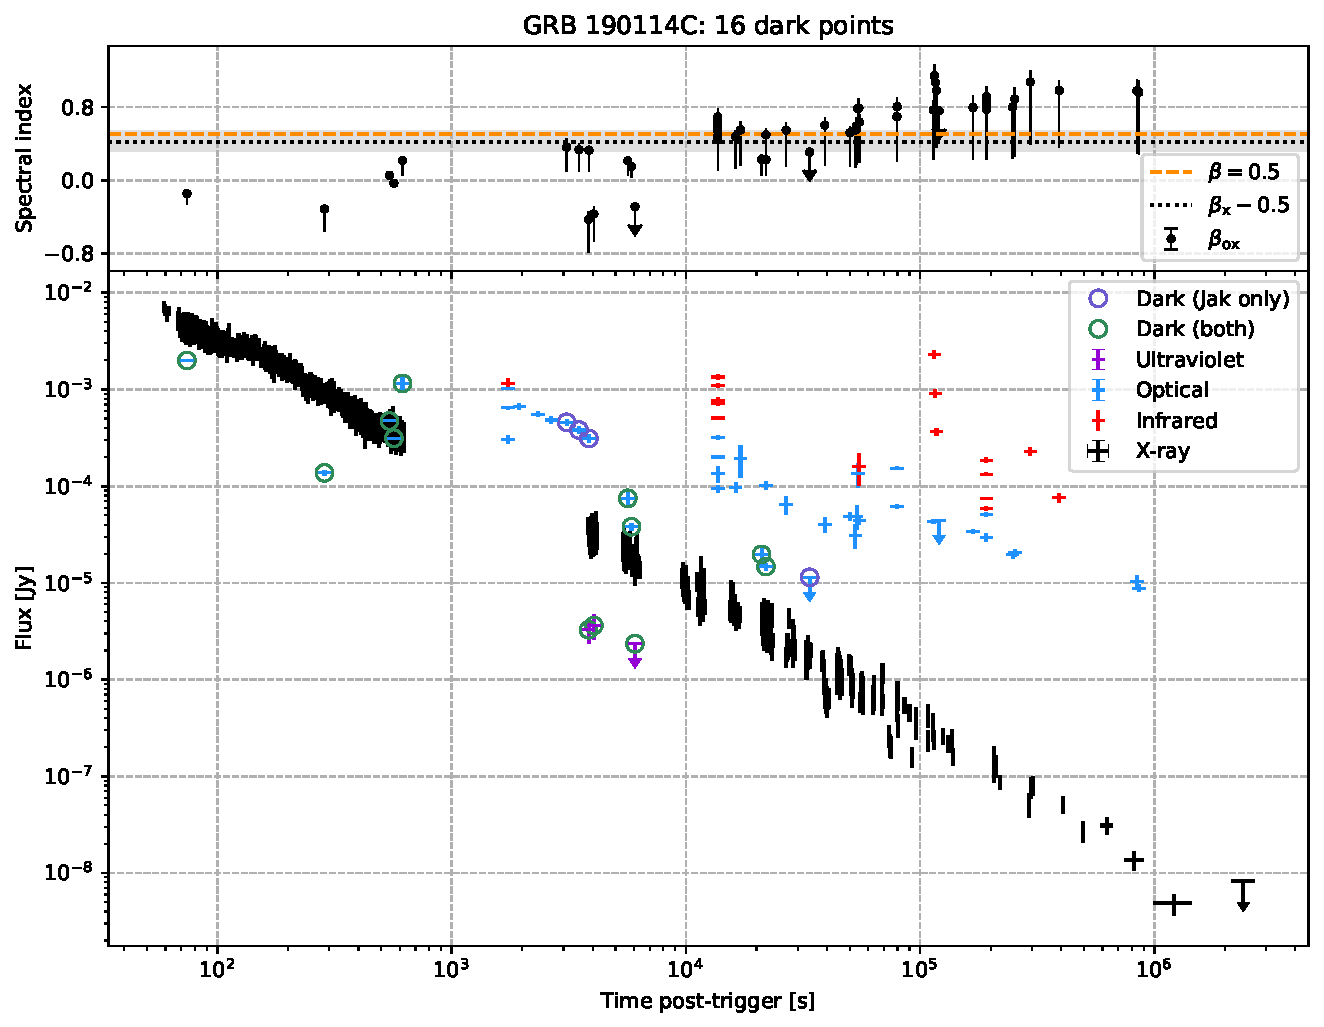
\includegraphics[width=0.90\linewidth]{figures/dark_lightcurves_190114C.pdf}
    \caption{Constructed light curve for GRB 190114C, where data from different energy regimes are plotted in different colors. Data is matched temporally within a tolerance of $\delta t = 20 \%$, from which $\beta_{ox}$ is calculated and plotted against the thresholds for optical darkness given by \cite{jakob} and \cite{opt_dark}. 16 dark points are found to be dark, so GRB 190114C is classified as a "dark burst."}
    \label{fig:light_curve}
\end{figure}

This work compares the $\beta_{ox}$ values of TeV GRBs to those of the larger long-duration GRB population to determine whether TeV bursts occur in systematically more obscured environments. X-ray afterglow data were obtained from the public Swift-XRT online repository provided by the UK Swift Science Data Centre (UKSSDC). Optical data were compiled from published literature, including circulars from NASA's Gamma-ray Coordinates Network (GCN) and peer-reviewed articles accessed through the SAO/NASA Astrophysics Data System (ADS).

For each TeV burst, I constructed light curves across the optical and X-ray energy regimes using my compiled data (see Fig.~\ref{fig:light_curve} for GRB 190114C and the Appendix for the other TeV GRBs). The UKSSDC provides integrated flux values across the entire XRT band (0.3--10 keV), so in order to compare fluxes at specific frequencies it was necessary to calculate the flux densities from these integrated fluxes. Assuming that the X-ray component of the afterglow spectrum is dependent on a single power-law with the spectral index $\beta_x$, this conversion is
\[
F_x = \int^{10 keV}_{0.3 keV} F_E \text{ d}E = A\int^{2.4 \times 10^{18} \text{Hz}}_{7.3 \times 10^{16} \text{Hz}} \nu^{-\beta_x} \text{ d} \nu,
\]

\noindent where $F_x$ is the UKSSDC-provided bolometric, or total, X-ray flux value and $A$ is a scaling coefficient that takes the burst's intrinsic X-ray luminosity as well as the distance from the burst into account. The analytical solution for the X-ray flux is therefore
\[
F_x =
\begin{cases}
    A\text{ ln}(\nu), & {\beta_x = 1} \\
    A \frac{\nu^{1-\beta_x}}{1-\beta_x}, & {\beta_x \neq 1}
\end{cases} 
\Biggl\}^{\nu = 2.4 \times 10^{18} \text{Hz}}_{\nu = 7.3 \times 10^{16} \text{Hz}} .
\]

To then solve for the flux at a specific frequency, $F_{\nu, x}$, one can utilize the relationship $A\nu^{-\beta_x}$ for the burst's unique value of $A$ and any frequency within Swift-XRT's detectable range. For this study, I selected $\nu$ to be $10^{\frac{\log(10) + \log(0.3)}{2}} \approx 1.732$ keV, or the logarithmic mid-point frequency of the telescope's 0.3--10 keV range. Optical fluxes were corrected, where possible, for galactic extinction using established extinction maps and normalized to common reference frequencies to enable direct comparison with X-ray measurements. All flux densities were converted to consistent units of janskys (Jy).

To compute $\beta_{ox}$, optical and X-ray flux densities were temporally matched by interpolating light curves to common epochs. The fractional temporal separation between optical observation time ($t_o$) and X-ray observation time ($t_x$) is defined by \cite{caden} as
\[
    \delta t_\% = \frac{|t_o - t_x|}{t_x},
\]

\noindent and this was computed for every combination of optical and X-ray data points within each GRB. Any pair satisfying $\delta t_\% \le 0.2$ was accepted as a candidate match. For each temporally matched pair, the broadband spectral index was calculated as
\[
    \beta_{ox} = \frac{\log(F_{\nu, opt} / F_{\nu,x})}{\log(\nu_{opt}/\nu_x)}.
\]

I classified bursts as being optically dark if $\beta_{ox}$ fell below the threshold defined relative to $\beta_{x}$, utilizing and cross-comparing both prescriptions by \cite{jakob} and \cite{opt_dark}. This approach enables identification of “dark points” within the light curve (as shown in Fig.~\ref{fig:light_curve}) and allows for direct comparison with the general long GRB population.



\subsection{Afterglow Spectral Modeling Analysis} \label{model_method}

\begin{figure}
    \centering
    % First subfigure
    \begin{subfigure}[b]{0.95\textwidth}
        \centering
        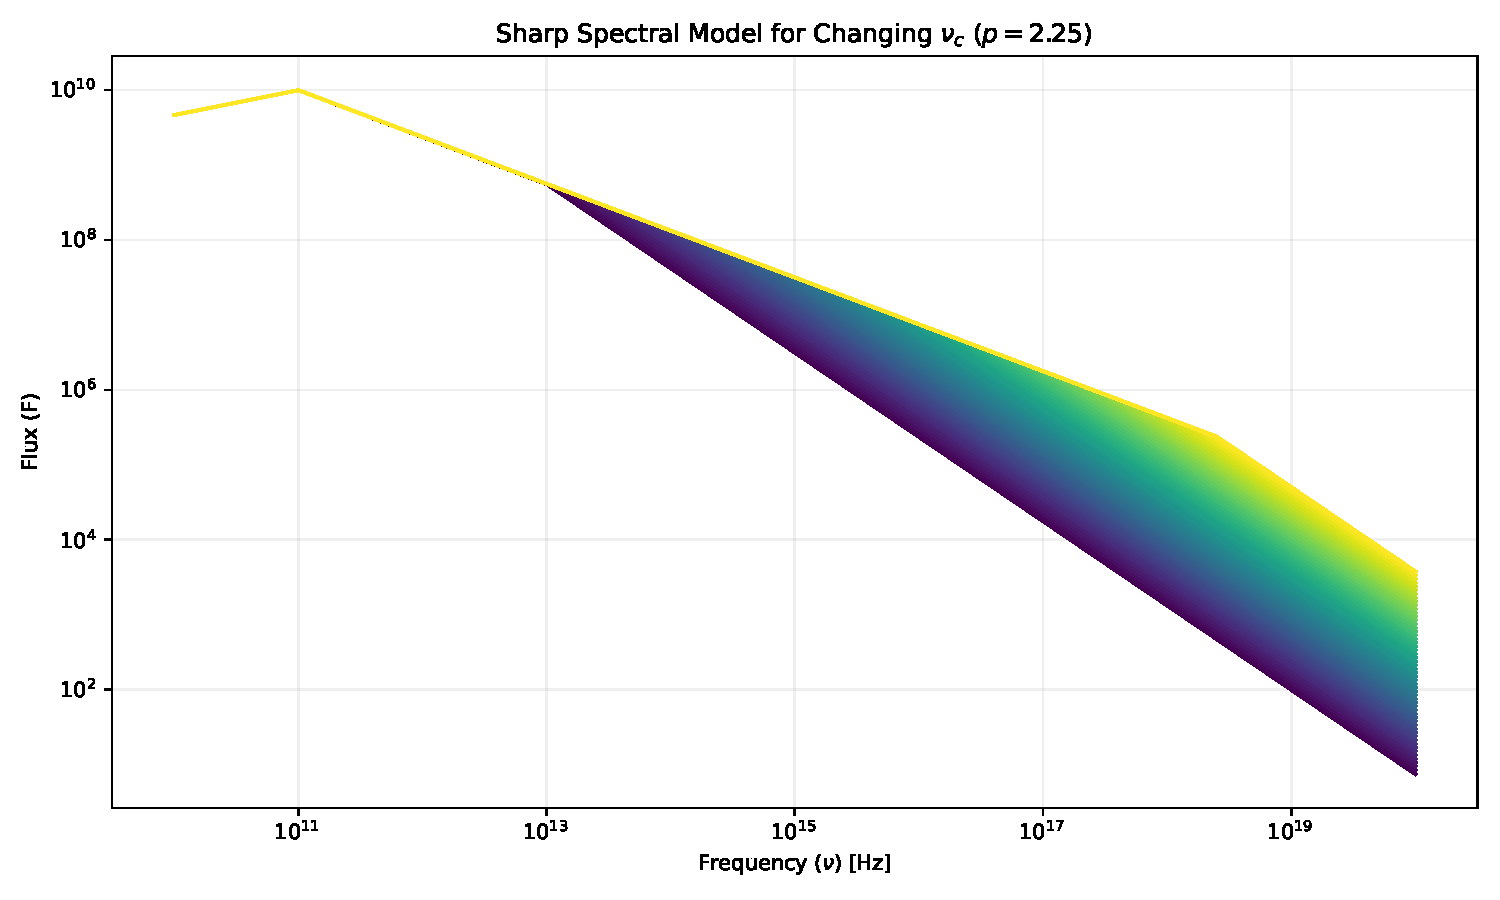
\includegraphics[width=\textwidth]{figures/sharp_spectra.pdf}
        \caption{Simulated Sharp-Break Spectrum}
        \label{fig:sharp}
    \end{subfigure}
    \hfill % Adds horizontal space
    % Second subfigure
    \begin{subfigure}[b]{0.95\textwidth}
        \centering
        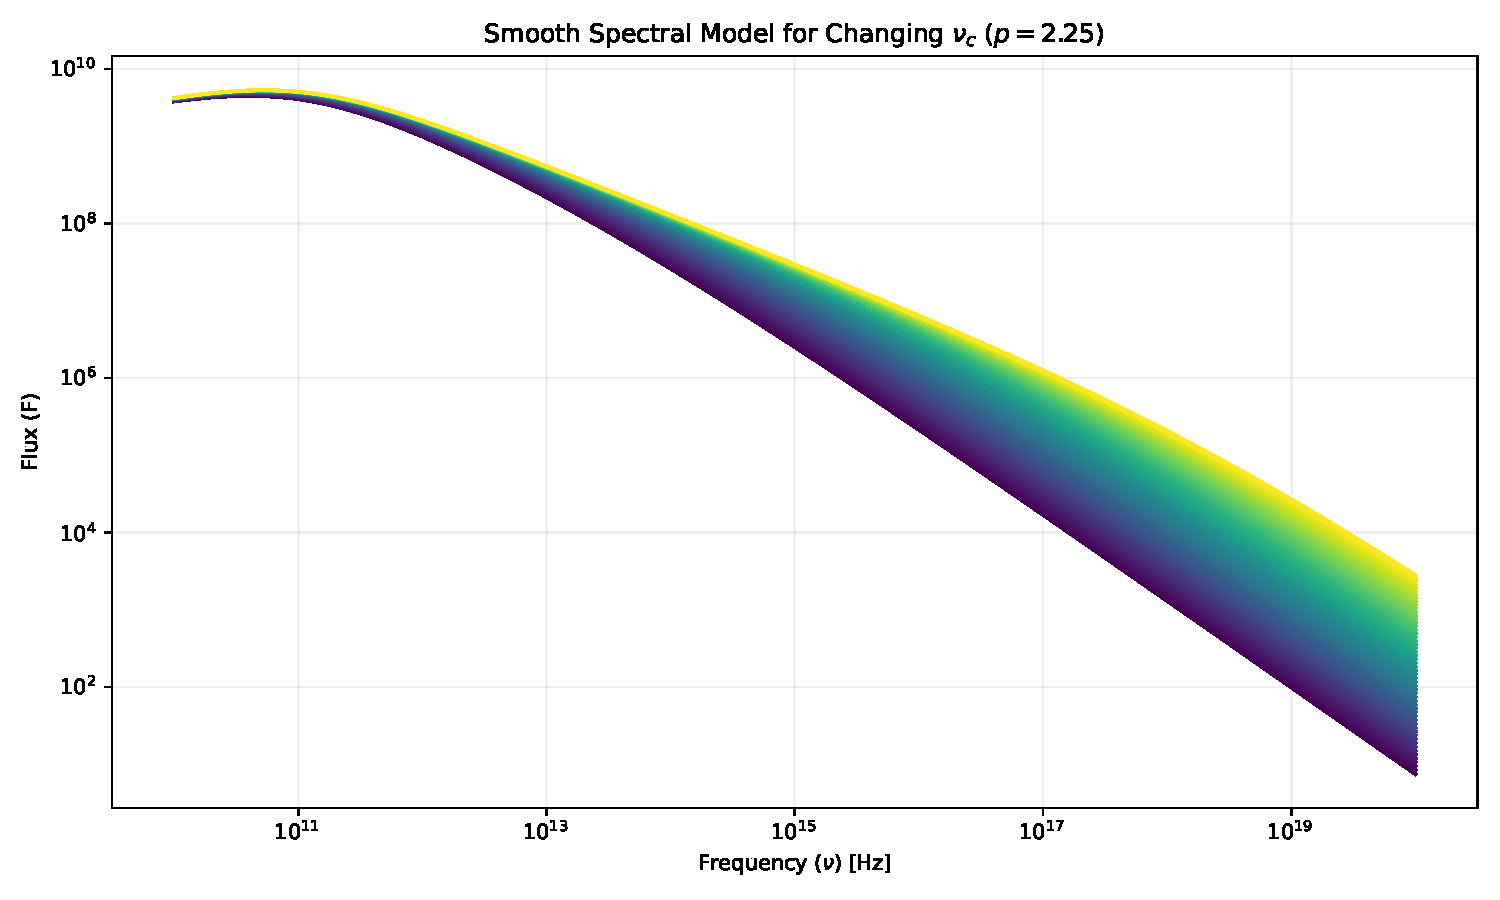
\includegraphics[width=\textwidth]{figures/smooth_spectra.pdf}
        \caption{Simulated Smooth-Break Spectrum}
        \label{fig:smooth}
    \end{subfigure}
    \caption{Sharp vs. Smooth Spectrum Models. The color gradient represents the evolution of the spectra with the changing location of the cooling break, $\nu_c$, starting with the navy blue where $\nu_c = 10^{13}$ Hz and ending with the yellow where $\nu_c = 10^{18.5}$ Hz.}
    \label{fig:sharp_v_smooth}
\end{figure}

The second component of this study focuses on the physics of particle acceleration and radiation in GRB jets by examining afterglow spectra across optical and X-ray wavelengths for a larger sample of bursts. In standard synchrotron afterglow theory, shock-accelerated electrons are described by a power-law energy distribution
\[
N(E) \propto E^{-p},
\]
where $p$ is the electron energy distribution index. The value of $p$ governs the the spectral and temporal slopes of the afterglow emission and therefore encodes fundamental information about particle acceleration in relativistic shocks \parencite{fireball}. Theoretical models of shock acceleration typically predict $p \sim 2.2$--2.3 \parencite{pvalues}, but observational studies have reported a range of values (such as $p=2.36$ with a width of $0.59$ according to \cite{other_pvalues}). Determining whether $p$ actually follows a universal distribution across the entire GRB population is crucial for testing particle acceleration theories and constraining underlying jet microphysics.

Standard analytical afterglow models approximate spectra using broken power laws that ``break,'' or sharply transition, at characteristic frequencies such as the electron cooling break, $\nu_c$. This electron cooling break is of particular importance as it serves as a threshold of electron energy in the afterglow. Electrons that have been accelerated in magnetic fields are the dominant source of afterglow radiation, and it is known that the more energetic an electron becomes the quicker it then loses, or radiates away, that energy. $\nu_c$ is the frequency corresponding to the energy where electrons begin to lose energy rapidly, beyond which we see a drastic fall off in the amount of radiation we detect from the source. Detailed numerical simulations, however, demonstrate that afterglow spectral transitions should be smoother and evolve continuously with time rather than exhibit the abrupt discontinuities we typically see at frequencies like $\nu_c$ \parencite{breaks}. Misidentification of break frequencies can introduce systematic errors in inferred physical parameters, particularly $p$.

This work addresses limitations with traditional spectral modeling by systematically analyzing multiwavelength spectral indices and implementing smoother spectral transitions. Spectral break frequencies, particularly $\nu_c$, are constrained by identifying transitions between the optical and X-ray energy regimes. Rather than assuming sharply broken power law relations, this study adopts a smoother parameterization of spectral curvature as discussed in \cite{breaks}, allowing for more realistic modeling of broadband spectra.

Sharply broken power-law spectra are modeled using the piecewise function:
\[
F(\nu) = 
     \begin{cases} 
      F_0 \left(\frac{\nu}{\nu_m}\right)^{\frac{1}{3}} & \nu \leq \nu_m \\
      F_0 \left(\frac{\nu}{\nu_m}\right)^{\frac{1-p}{2}} & \nu_m < \nu \leq \nu_c \\
      F_0 \left(\frac{\nu_c}{\nu_m}\right)^{\frac{1-p}{2}} \left(\frac{\nu}{\nu_c}\right)^{-\frac{p}{2}} & \nu > \nu_c 
    \end{cases}
\]
where $F_0$ is a normalization constant, $\nu$ is the observing frequency, $\nu_m$ is the characteristic synchrotron frequency (fixed at $10^{11}$ Hz for this study as we focus on the slow cooling, or later time, regime), $\nu_c$ is the electron cooling break frequency (varied logarithmically between $10^{13}$ and $10^{18.5}$ Hz), and $p$ is the electron energy distribution index (fixed at 2.25, the midpoint of the range proposed by \cite{pvalues}). Figure~\ref{fig:sharp} shows the evolution of spectra generated across a frequency range of $10^{10}$--$10^{20}$ Hz for different values of $\nu_c$.

For smoothly broken spectra, I adopt the prescription of \cite{breaks}:
\[
F(\nu) = F_0 \left[\left(\frac{\nu}{\nu_m}\right)^{-\frac{s_m}{3}} + \left(\frac{\nu}{\nu_m}\right)^{-\frac{s_m(1-p)}{2}}\right]^{-\frac{1}{s_m}} \left[1 + \left(\frac{\nu}{\nu_c}\right)^{\frac{s_c}{2}}\right]^{-\frac{1}{s_c}},
\]
where $F_0$, $\nu_m$, and $\nu_c$ are defined as above with the sharp-break model. The sharpness parameters are given by
\[
s_m = 2.2 - 0.52p, \quad
s_c = 1.6 - 0.38p - 0.16k + 0.078pk,
\]
where $k$ describes the circumburst density profile ($k=0$ for a constant-density interstellar medium and $k=2$ for a stellar wind environment). Adopting $p = 2.25$ as I did with the sharp model and $k = 0$, I obtain $s_m = 1.030$ and $s_c = 0.745$. Figure~\ref{fig:smooth} illustrates the resulting smoothly broken spectra.

To constrain spectral break locations, I generated spectra using both the sharp and smooth models for $\nu_c$ values ranging from $10^{13}$ to $10^{18.5}$ Hz. I then compared them to observed, time-integrated optical and X-ray spectral indices from a sample of 105 GRBs pulled from \cite{grb_sample}'s catalogue. The position of $\nu_c$ directly influences the observed optical ($\beta_o$) and X-ray ($\beta_x$) spectral slopes, and therefore the calculated broadband index $\beta_{ox}$. The primary goal of this comparison is to determine whether the use of the smooth-break model with variations in $\nu_c$ can account for the observed diversity in spectral indices while maintaining a universal value of $p$ \parencite{granot_smooth}. If successful, this would support standard GRB afterglow theory while providing a more physically motivated method for identifying cooling break frequencies. Additionally, comparing sharp and smooth spectral models allows for a direct test of whether smooth transitions provide a better representation of observed afterglow spectra as predicted by numerical simulations \parencite{breaks}.

\begin{figure} [t]
    \centering
    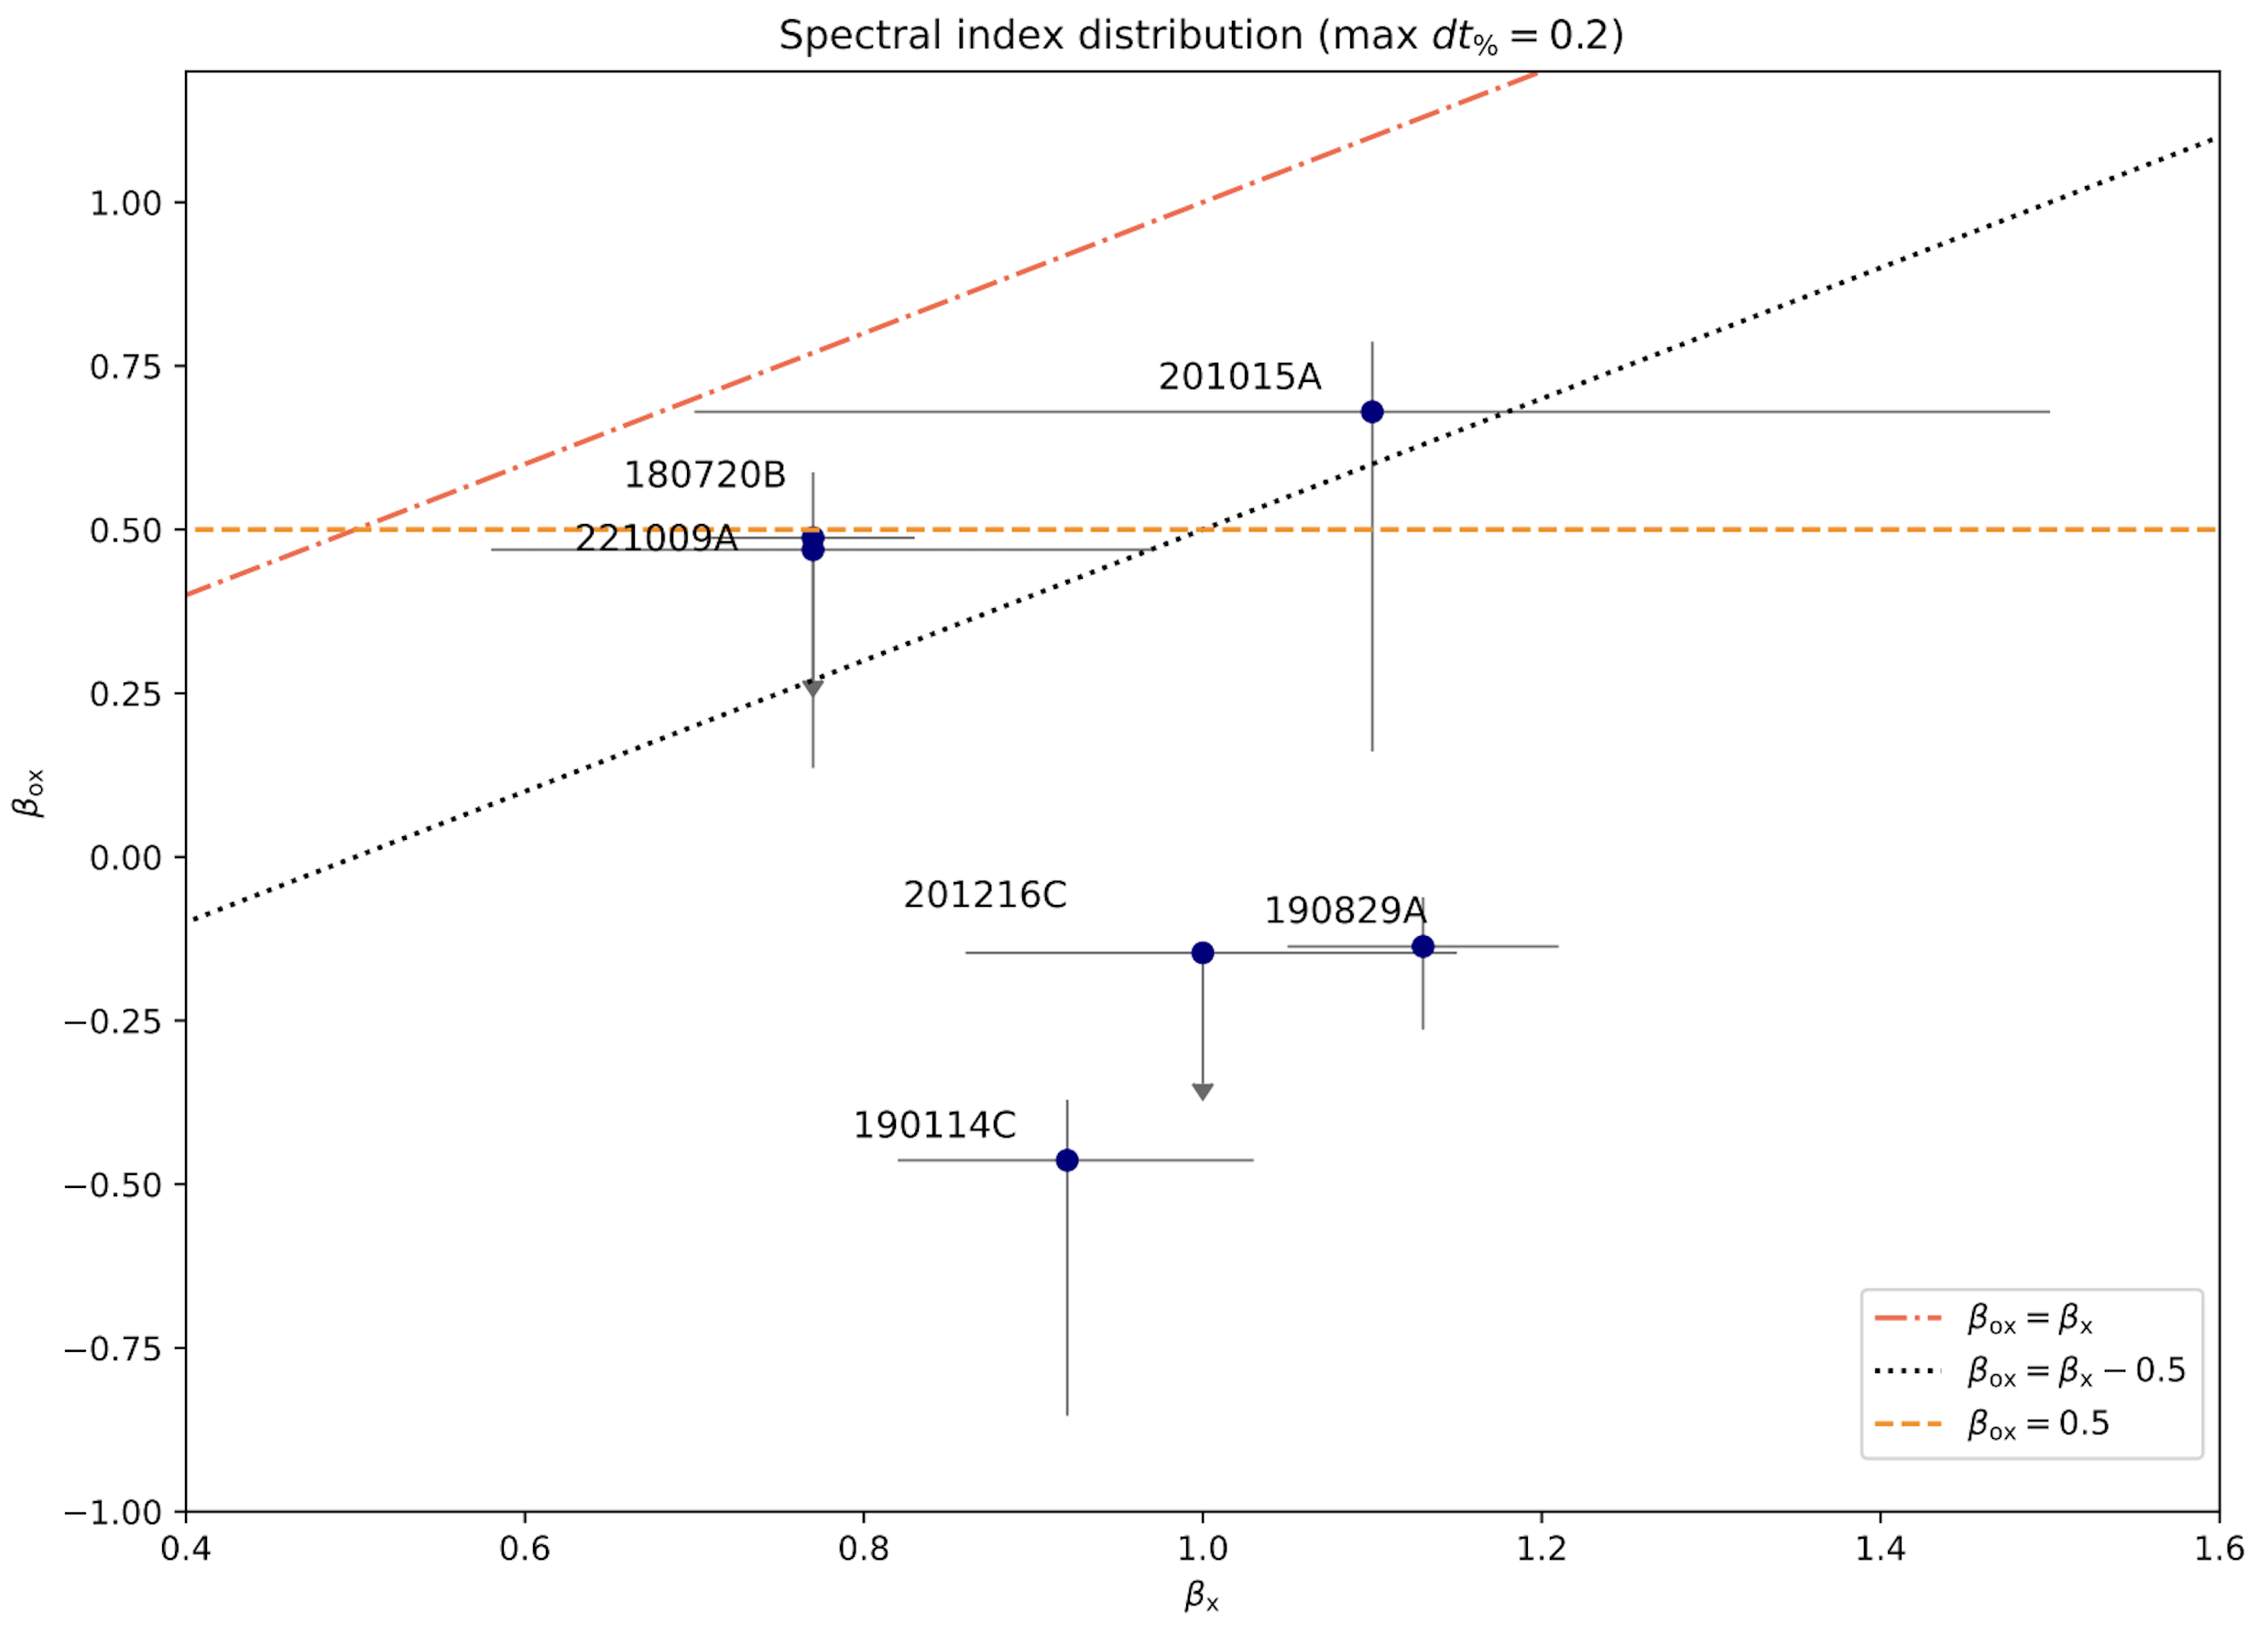
\includegraphics[width=0.80\linewidth]{figures/opt_dark_results.png}
    \caption{$\beta_{ox}$ vs $\beta_x$ for TeV GRBs compared to optical darkness thresholds defined by \cite{jakob} (dashed light orange line) and \cite{opt_dark} (dotted black line). The dark orange line represents the case where $\beta_{ox} = \beta_{x}$. This plot shows that GRBs 190114C, 190829A, and 201216C are optically dark as they fall below the dotted black line, while GRBs 180720B, 201015A, and 221009A are not because they lie above.}
    \label{fig:opt_dark}
\end{figure}

\section{Results}

\subsection{TeV GRB Optical Darkness Analysis Results}

Using temporally matched optical and X-ray flux densities, I calculated $\beta_{ox}$ for each of the six TeV GRBs in the sample. Applying the optical darkness criteria from \cite{opt_dark}, three bursts (GRBs 190114C, 190829A, and 201216C) are clearly classified as optically dark, while three bursts (GRBs 180720B, 201015A, and 221009A) are not (see Fig.~\ref{fig:opt_dark} for a comparison of $\beta_{ox}$ and $\beta_x$ for all TeV GRBs).


This classification is broadly consistent with the earlier definition from \cite{jakob}, although that framework places GRBs 180720B and 221009A near the boundary of dark vs. non-dark classifications. To resolve this ambiguity, I examined the full multiwavelength light curves for each burst and identified any temporally matched optical--X-ray spectral index pairs satisfying $\delta t_\% \leq 0.2$. A clear separation emerges when considering the number of dark data points. GRBs classified as optically dark exhibit multiple dark epochs (16 for GRB 190114C, 19 for GRB 190829A, and 8 for GRB 201216C), indicating persistent optical suppression over time (for example, see the upper plot in Fig~\ref{fig:light_curve}). The non-dark bursts, by constrast, show zero dark points under the same temporal matching criteria. This strengthens the robustness of their classification by demonstrating that the exhibited optical darkness is not driven by isolated measurements and instead reflects a sustained broadband property of the afterglow. Overall, 3 out of the 6 TeV GRBs observed thus far are optically dark, though the small sample size limits the statistical significance of this result.


\subsection{Afterglow Spectral Modeling Results}

\begin{figure} [t]
    \centering
    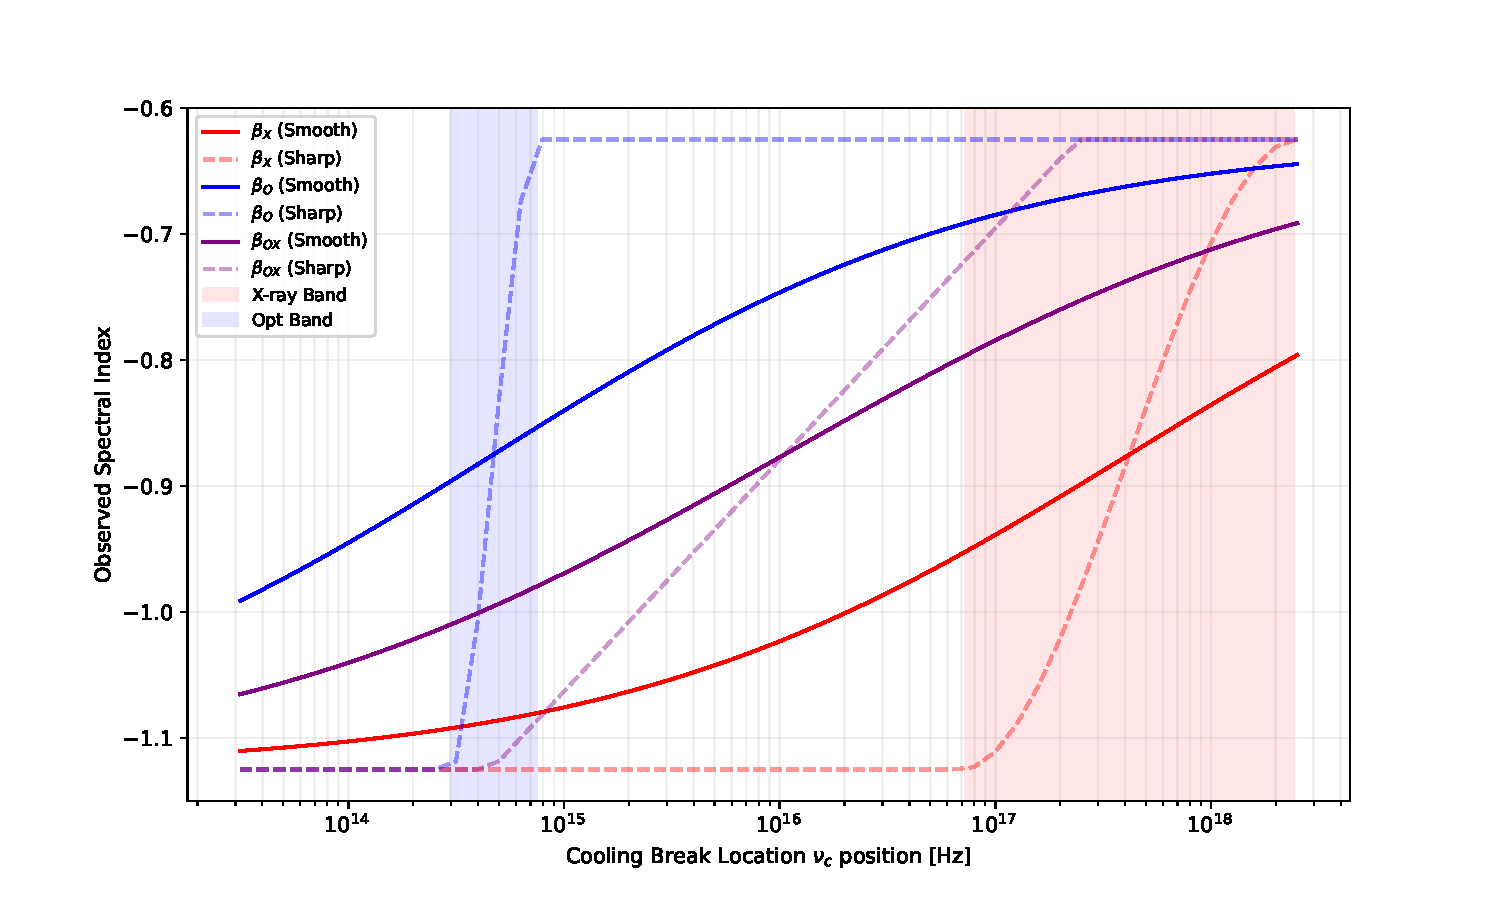
\includegraphics[width=1.00\linewidth]{figures/spectral_indices.pdf}
    \caption{Evolution of spectral indices $\beta_o$, $\beta_x$, and $\beta_{ox}$ (blue, red, and purple respectively) as a function of the location of the cooling break frequency, $\nu_c$. The dashed lines correspond to the sharp-break model while the solid lines correspond to the smooth-break model. The blue and red shaded regions represent the optical and X-ray frequency bands respectively.}
    \label{fig:spectral_indices}
\end{figure}

\begin{figure} [h]
    \centering
    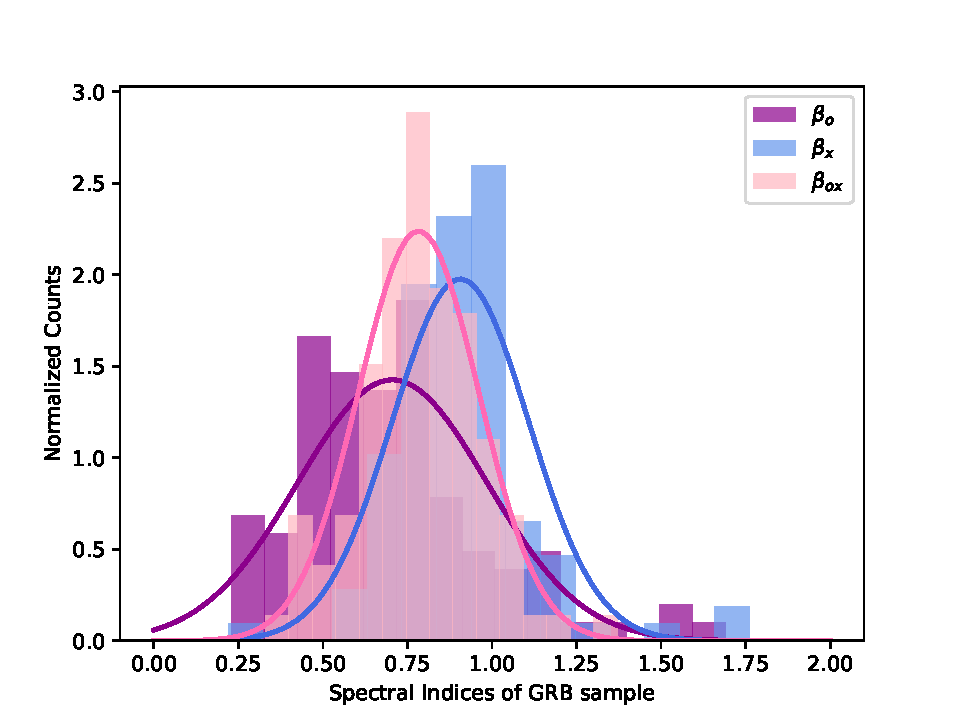
\includegraphics[width=0.75\linewidth]{figures/spectral_indices_hist.pdf}
    \caption{Observed time-integrated spectral indices $\beta_o$ (shown in purple) and $\beta_x$ (shown in light blue), and calculated broadband index $\beta_{ox}$ (shown in light pink), from sample of 105 GRBs. All are fitted with Gaussian distributions to determine their means and standard distributions.}
    \label{fig:spec_ind_figs}
\end{figure}

My simulations of afterglow spectra using an assumed universal value of $p=2.25$ confirm that the inferred spectral indices $\beta_o$ and $\beta_x$, and the calculated broadband $\beta_{ox}$, depend strongly on the location of the cooling break frequency, $\nu_c$, as well as on the assumed spectral model. For sharply broken power-law spectra, the behavior of the spectral indices is highly discontinuous. The values of $\beta_o$ and $\beta_x$ remain constant until $\nu_c$ passes through the corresponding observational band (optical or X-ray), at which point they change abruptly (see Fig.~\ref{fig:spectral_indices}). This produces a step-like transition in the spectral indices that reflects the unphysical nature of the imposed spectral breaks. By contrast, the smoothly broken power-law model produces a continuous evolution in all spectral indices as $\nu_c$ varies. Both $\beta_o$ and $\beta_x$ continue to gradually evolve even when $\nu_c$ lies outside the observed bands due to the extended curvature of the spectrum. As a result, $\beta_{ox}$ also evolves smoothly without discontinuities. A key result is that the smooth model predicts an intermediate range of spectral slopes that are less accessible in the sharp-break approximation. 

I also compared the smooth-break model to the average values of the spectral indices I gathered for my 105 GRB sample from \cite{grb_sample}'s catalogue (see Fig.~\ref{fig:spec_ind_figs} for distribution of spectral indices from data and Fig.~\ref{fig:spectral_indices_w_data} for comparisons to simulation). With this model, I find an overlap in the average values of $\beta_o$, $\beta_{ox}$, and $\beta_x$ (given in Table~\ref{tab:spec_ind} along with their standard deviations) with an electron cooling break, $\nu_c$, located near the lower end of the X-ray energy band. This overlap across the different spectral indices does not occur with the sharp-break model due its discontinuous nature.

I am also confident that these spectral indices are distinct and not from the same parent distribution despite their large standard deviations. I performed a Kolmogorov-Smirnov (KS) statistical test comparing both $\beta_o$ and $\beta_x$ as well as $\beta_o +0.5$ and $\beta_x$, finding probability values of $4.66 \cdot 10^{-12}$ and $4.51 \cdot 10^{-15}$ respectively. As both of these p-values are extremely small, this test proves that $\beta_o$ and $\beta_x$ are distinct distributions, and can therefore be compared separately to my simulated spectral indices in Fig.~\ref{fig:spectral_indices_w_data}.


\begin{table}[h]
\centering
    \begin{tabular}{|Sc|Sc|Sc|}
    \hline
    Spectral Index ($\beta$)              & Average ($\mu$) & Standard Deviation ($\sigma$) \\ 
    \hline
    $\beta_o$      & 0.71    & 0.28               \\ 
    \hline
    $\beta_{ox}$ & 0.78    & 0.18               \\ 
    \hline
    $\beta_x$      & 0.91    & 0.20              \\ 
    \hline
    \end{tabular}
    \caption{The average values and corresponding standard deviations of the spectral indices $\beta_o$, $\beta_{ox}$, and $\beta_x$ for the sample of 105 GRBs pulled from \cite{grb_sample}'s GRB catalogue.}
    \label{tab:spec_ind}
\end{table}


\section{Discussion}


\subsection{TeV GRB Optical Darkness Discussion}

The fraction of optically dark bursts in the TeV GRB subset (50\%) is generally consistent with the $\sim$40\% fraction reported for the general long GRB population \parencite{40_percent}. Although the sample size is small, this agreement suggests that TeV GRBs do not preferentially occur in unusually dust-rich or optically obscured environments as they do not display the corresponding optical extinction. This result has important implications for understanding the origin of very high-energy GRB emission. If dense or dusty environments were the primary driver of TeV emission, either through the enhancement of synchrotron self-Compton scattering or the modification of shock conditions, one would expect TeV GRBs to exhibit a systematically higher rate of optical darkness. The absence of such a trend indicates that environmental factors alone are unable to explain their extreme energetics. To ensure that this result is robust, it is also important to consider potential observational biases. In particular, early-time afterglow emission can be affected by prompt emission contamination or rapid spectral evolution, which may artificially suppress optical fluxes or lead to an X-ray excess \parencite{early_afterglow, liang, nousek}. By requiring temporal matching within $\delta t_\% \leq 0.2$ and identifying multiple dark epochs per burst, particularly after a threshold of 5 minutes (300 seconds) post-burst established by \cite{caden} and in regions where the X-ray behavior is canonical and therefore absent of flares or plateaus, this analysis minimizes the likelihood that individual dark points are driven by such transient effects.

This result also motivates the exploration of other hypotheses, such as the possibility that TeV GRBs are not intrinsically distinct from the broader GRB population, but rather have only recently become observable due to advances in high-energy instrumentation. Facilities such as ground-based Cherenkov telescopes have significantly improved sensitivity in the TeV regime, enabling the detection of emission that may in reality be common but was previously inaccessible \parencite{sitarek}. Under this scenario, TeV emission may be a generic feature of GRB afterglows rather than a signature of a rare subclass, with detectability governed by instrumental limitations and observational conditions. Future observations will be critical in resolving this question. Expanding the sample of TeV GRBs and obtaining more uniform multiwavelength coverage will allow for more statistically significant comparisons and help distinguish intrinsic physical differences from observational selection effects.


\subsection{Afterglow Spectral Modeling Discussion}

\begin{figure} [t]
    \centering
    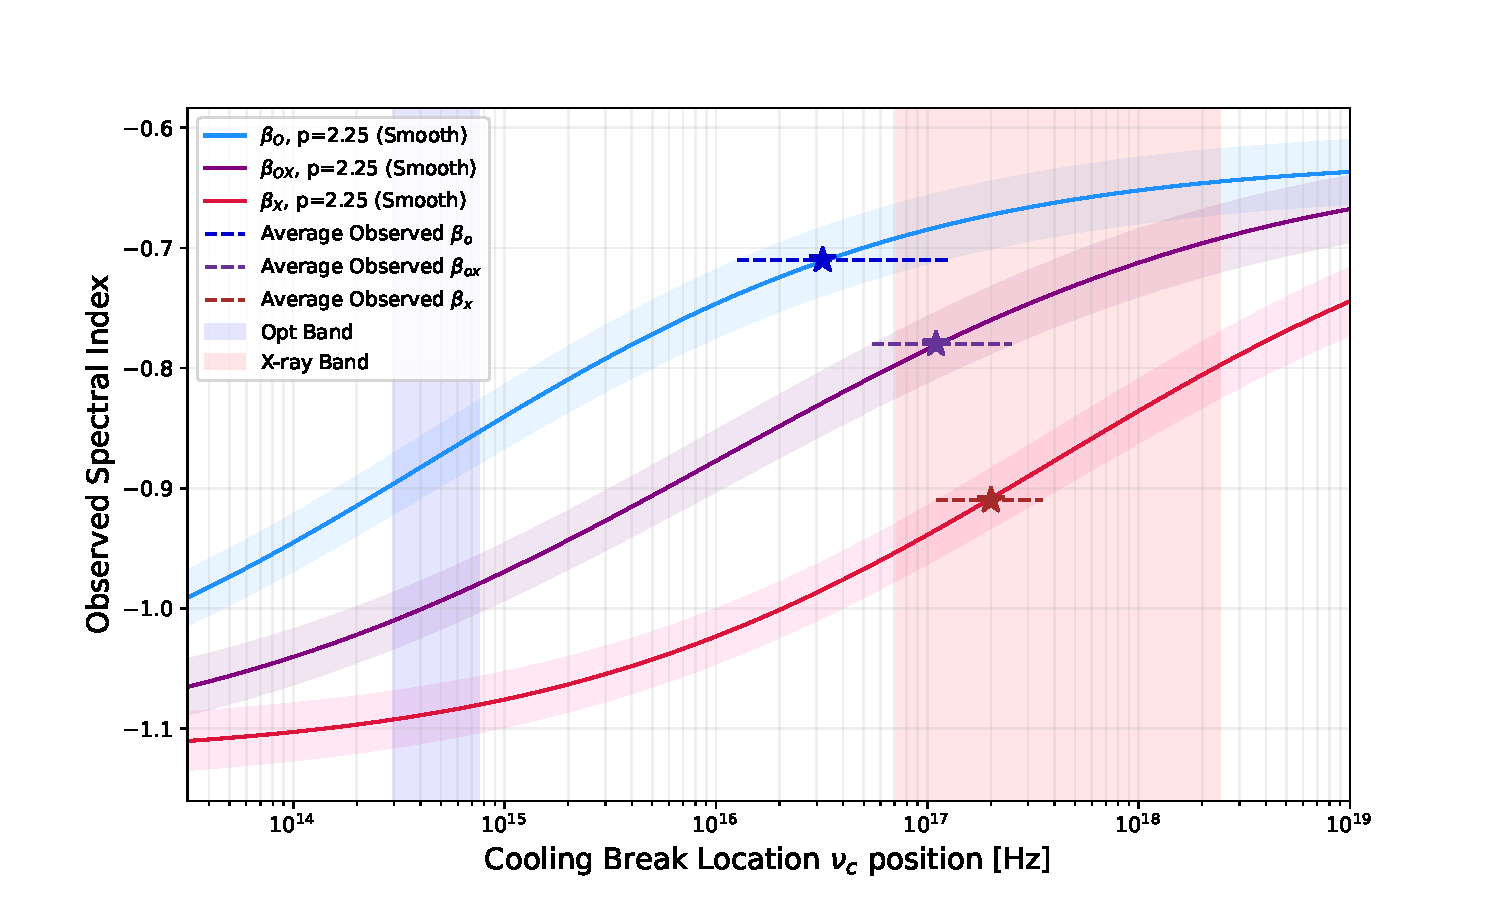
\includegraphics[width=0.90\linewidth]{figures/spectral_indices_stars_poster.pdf}
    \caption{Comparison of smooth-break spectral model to the average observed spectral indices (indicated by the star markers and corresponding dotted lines) from the 105 GRB sample. The shaded regions around each index represents the index values associated with a narrow $p$ range of 2.2--2.3. From this preliminary comparison, we can see that $\nu_c$ likely lies near or in the lower end of the X-ray band.}
    \label{fig:spectral_indices_w_data}
\end{figure}

The results of the spectral modeling analysis demonstrate that the treatment of spectral breaks has a significant impact on the interpretation of GRB afterglow data. The commonly used sharp broken power-law approximation introduces unphysical discontinuities in spectral indices, which can lead to biased or oversimplified inferences about physical parameters. In particular, the sharp-break model restricts spectral indices to nearly discrete values determined solely by the location of $\nu_c$ within the optical and X-ray bands observational bands. This can obscure the true underlying behavior of the spectrum and lead to the misidentification of the cooling break frequency. In contrast, the smoothly broken model produces a continuous spectral evolution, allowing for coincident intermediate slopes that more accurately reflect physical expectations from synchrotron radiation theory \parencite{pvalues}.

One important implication of this result is that the observed diversity in spectral indices across GRBs \parencite{other_pvalues, starling, ryan} does not necessarily require a broad distribution of the electron energy index $p$. Instead, a significant fraction of this variation can be explained by differences in the location of $\nu_c$ and a smooth curvature of the spectrum. This supports the possibility that $p$ may be closer to a universal value than previously inferred by \cite{other_pvalues, starling}, and \cite{ryan} which is consistent with theoretical predictions from relativistic shock acceleration \parencite{pvalues}.

Additionally, confirming that $\beta_o$ and $\beta_x$ arise from separate distributions through a KS-test supports the use of the smooth-break model. The sharp-break model, assuming a constant value of $p$, requires that the optical and X-ray spectral indices should differ by a constant value of 0.5, but I found that the average $\beta_o$ and $\beta_x$ only differ by 0.2. This sort of difference can only be seen with a smoother spectral model that can access intermediate spectral slopes. Furthermore, the smooth spectral model provides a more reliable framework for locating the cooling break. Because $\beta_o$, $\beta_x$, and $\beta_{ox}$ evolve gradually with $\nu_c$, it becomes possible to constrain the break frequency even when it lies outside the optical and X-ray observational bands. This represents a significant improvement over traditional methods, which rely on identifying sharp transitions that may not exist in real data. These findings highlight the importance of incorporating physically motivated spectral shapes into afterglow modeling. Future work should extend this approach by fitting smooth spectral models directly to observational data and exploring how inferred parameters such as $p$ and $\nu_c$ depend on the assumed spectral form. Such analyses will be essential for developing a more accurate and self-consistent picture of particle acceleration and radiation in GRB jets. 



\section{Conclusion}

In this work, I investigated two key aspects of GRB physics, from the role of the circumburst environment in producing very high-energy (TeV) emission to the impact of spectral modeling assumptions on the interpretation of afterglow observations. Through an analysis of optical darkness in the six TeV GRBs detected thus far, I found that half of the sample can be classified as optically dark. This fraction is consistent with that observed in the broader long GRB population (with 40\% being optically dark), indicating that TeV GRBs do not preferentially occur in unusually dust-rich or highly obscured environments. This result suggests that environmental effects alone are unlikely to be the dominant factor driving their extreme energetics. Instead, another hypothesis predicts that TeV emission may be a more generic feature of GRB afterglows that has only recently become observable due to advances in high-energy instrumentation.

The second part of this study demonstrates that the interpretation of GRB afterglow spectra depends sensitively on how spectral breaks are modeled. Traditional sharply broken power-law models introduce unphysical discontinuities in spectral indices, whereas smoothly broken models predict continuous spectral evolution as a function of the cooling break frequency, $\nu_c$. I show that variations in $\nu_c$ with this smooth model can naturally reproduce a wide range of observed spectral indices without requiring large intrinsic variations in the electron energy distribution index, $p$. This supports the possibility that $p$ may be closer to a universal value than previously inferred from GRB observations, ultimately supporting high-energy astrophysics theory \parencite{pvalues}. These findings highlight the importance of adopting physically motivated spectral models when analyzing GRB afterglows. Future work should focus on fitting smooth spectral models directly to multiwavelength data, and incorporating the use of time-resolved spectral index measurements to investigate the temporal evolution of $\nu_c$. Such efforts will be essential for developing a more complete understanding of particle acceleration, radiation mechanisms, and jet dynamics in some of the most extreme environments in the universe.


\printbibliography


\section{Acknowledgments}

\noindent I would like to thank my advisor Dr. Alexander van der Horst for his guidance and support throughout these projects, his feedback and our conversations have been invaluable. I would also like to acknowledge Dr. van der Horst and Dr. Axel Schmidt as my research advisors; I have learned an incredible deal under their mentorship and for that I am deeply grateful. I would also like to thank the GW Department of Physics for being such a wonderfully supportive environment that I am proud to have been a part of.

\section{Appendix} 

\vspace{4.0cm}

\begin{figure} [h]
    \centering
    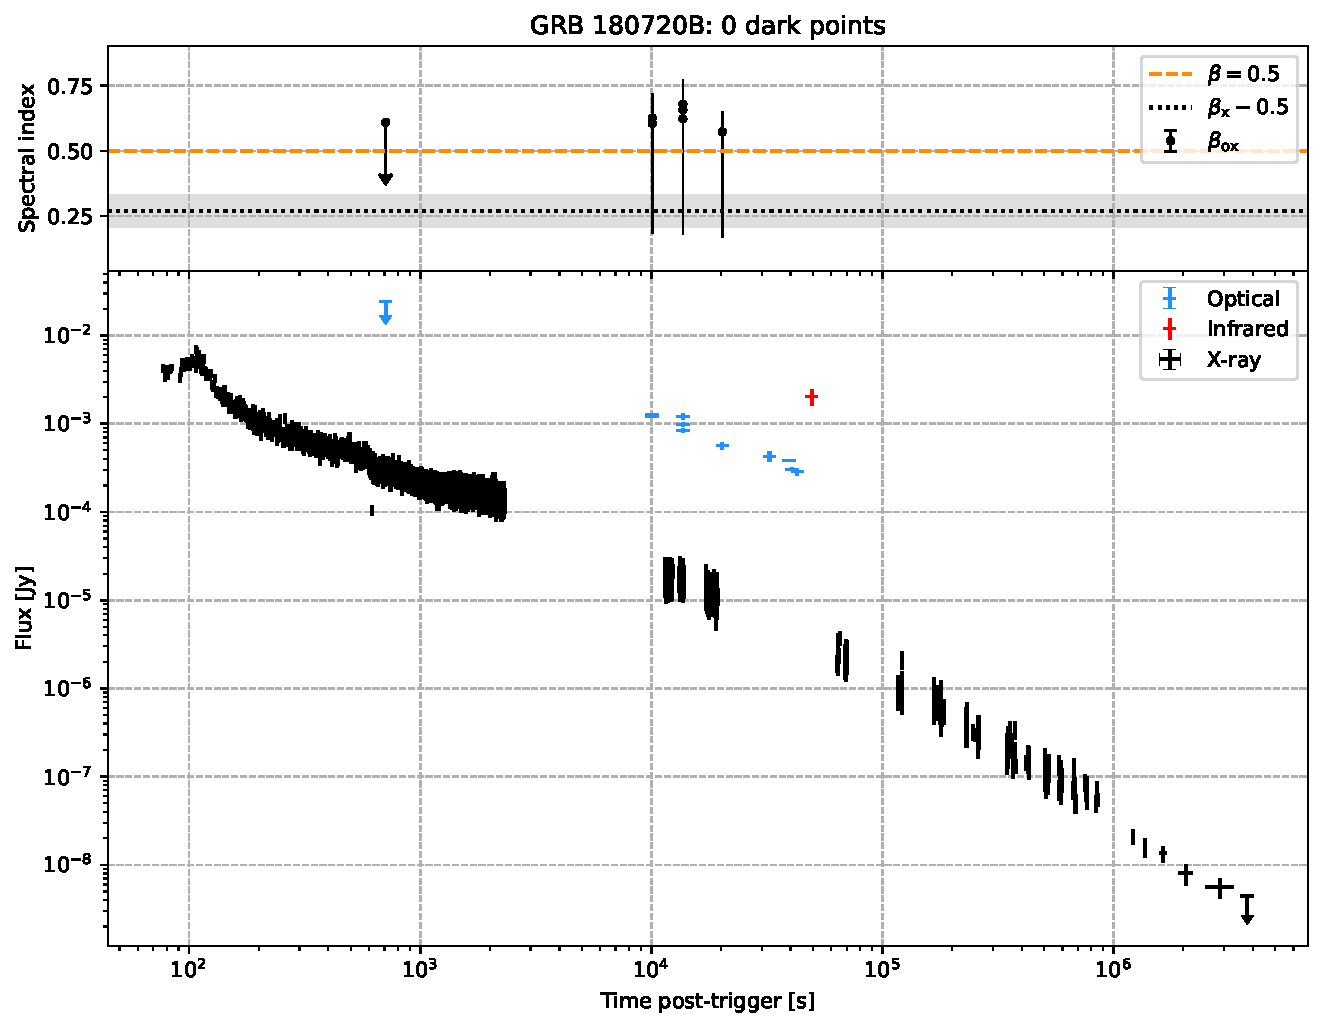
\includegraphics[width=0.80\linewidth]{appendix_figures/dark_lightcurves_180720B.pdf}
    \caption{Constructed light curve for GRB 180720B.}
    \label{180720B}
\end{figure}

\begin{figure} [h]
    \centering
    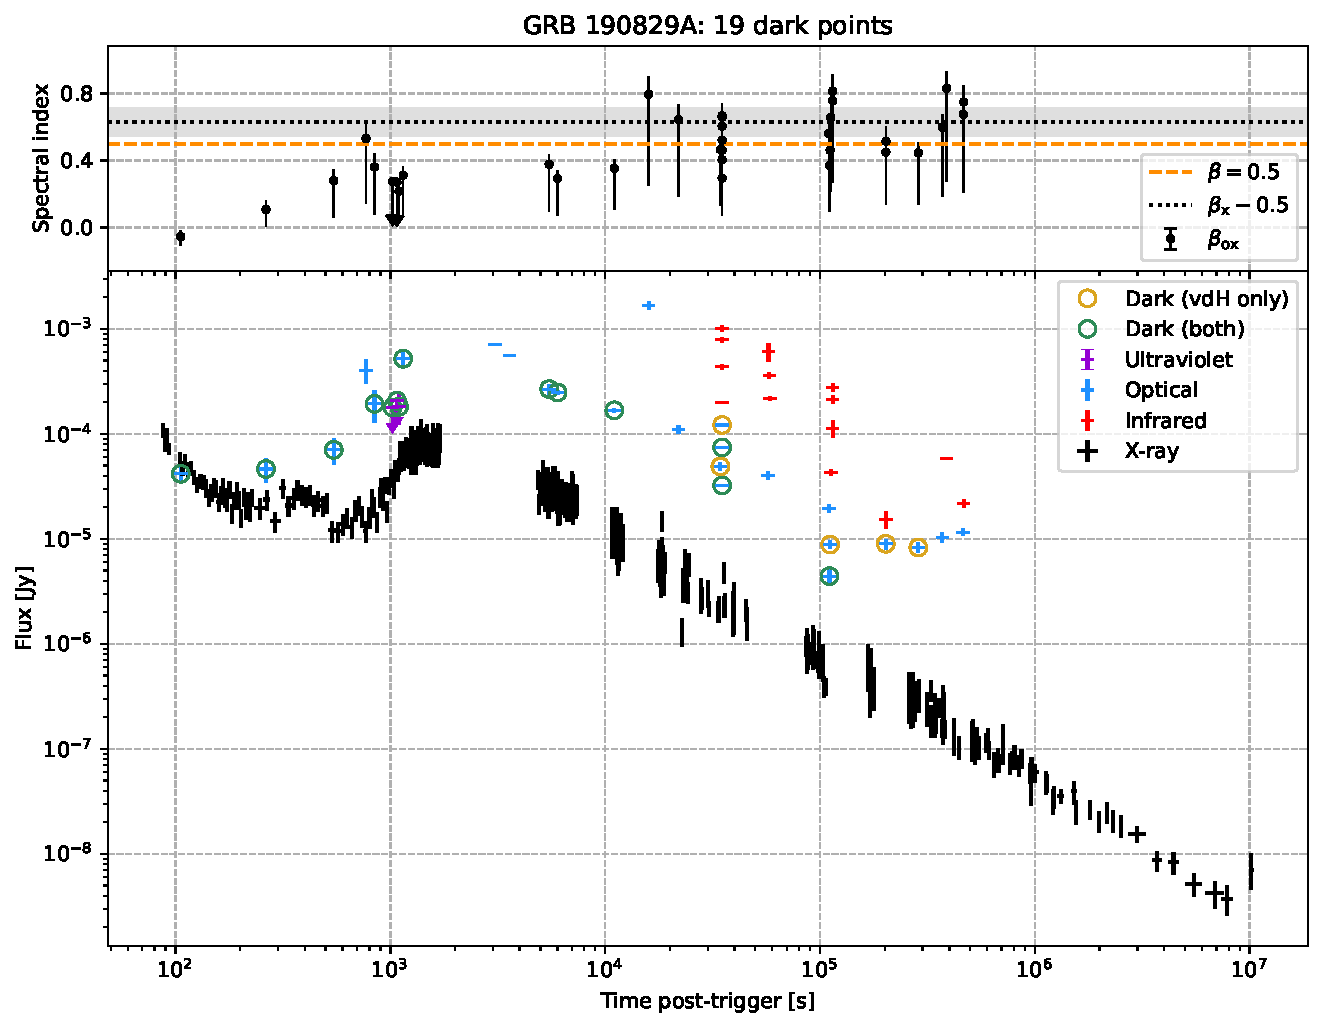
\includegraphics[width=0.80\linewidth]{appendix_figures/dark_lightcurves_190829A.pdf}
    \caption{Constructed light curve for GRB 190829A.}
    \label{190829A}
\end{figure}


\begin{figure} 
    \centering
    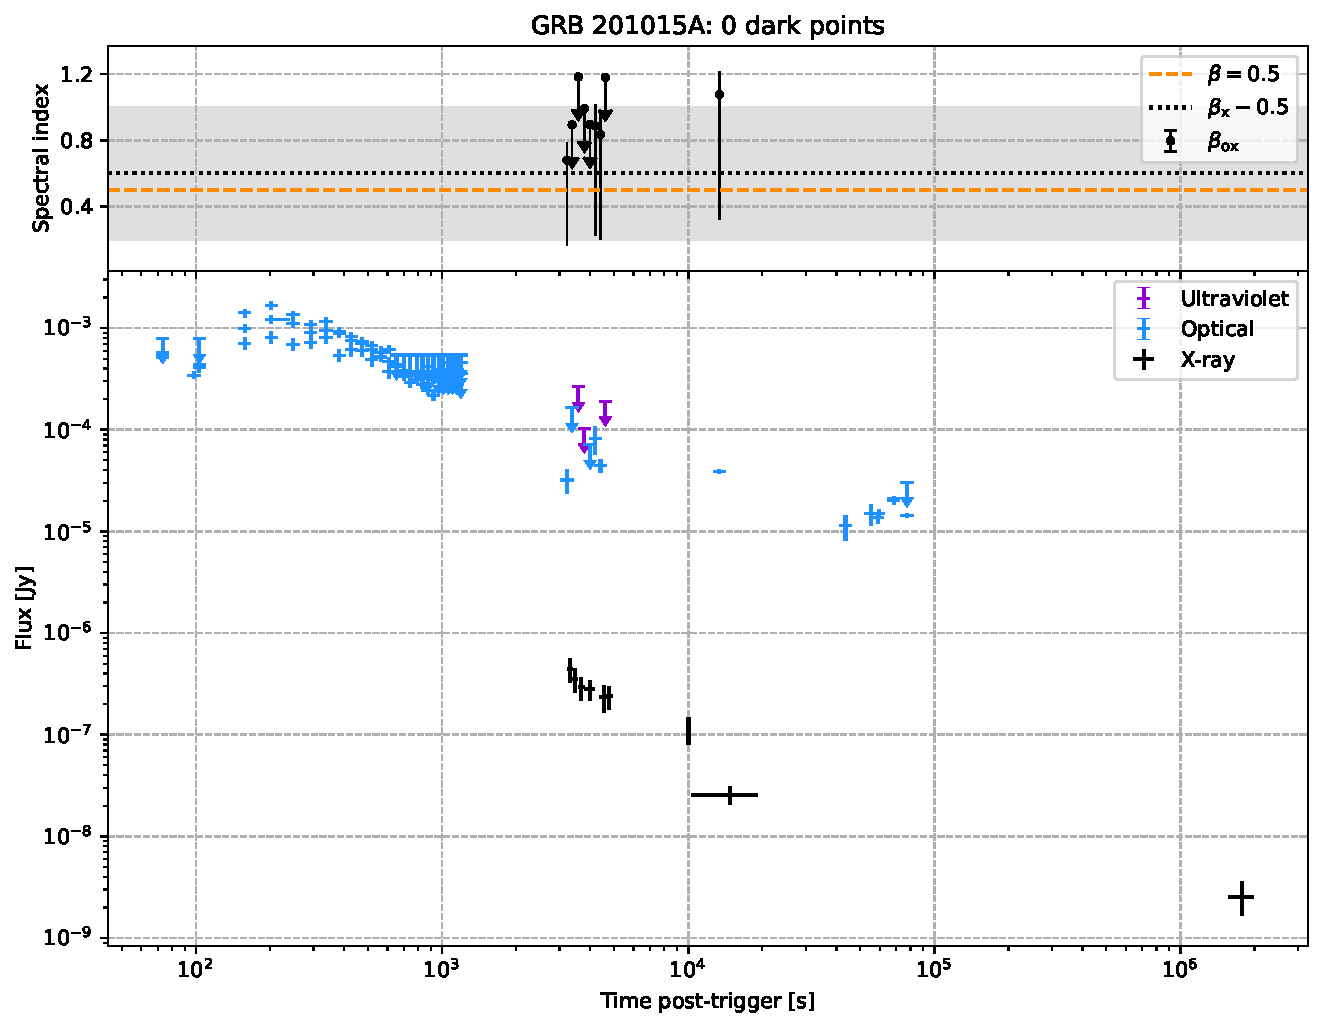
\includegraphics[width=0.80\linewidth]{appendix_figures/dark_lightcurves_201015A.pdf}
    \caption{Constructed light curve for GRB 201015A.}
    \label{201015A}
\end{figure}

\begin{figure} 
    \centering
    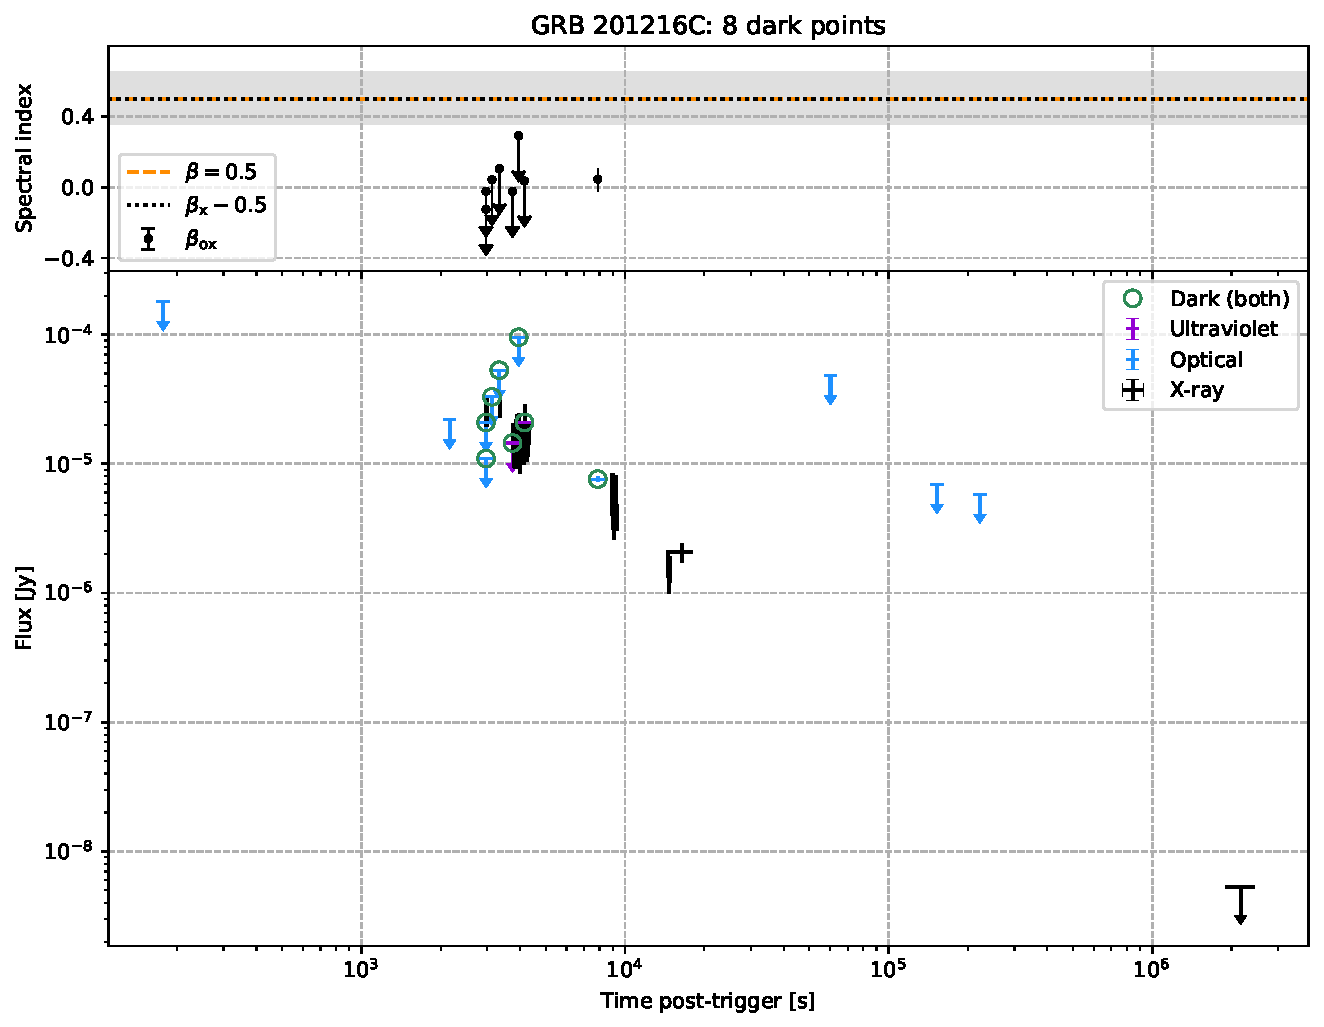
\includegraphics[width=0.80\linewidth]{appendix_figures/dark_lightcurves_201216C.pdf}
    \caption{Constructed light curve for GRB 201216C.}
    \label{201216C}
\end{figure}

\begin{figure}
    \centering
    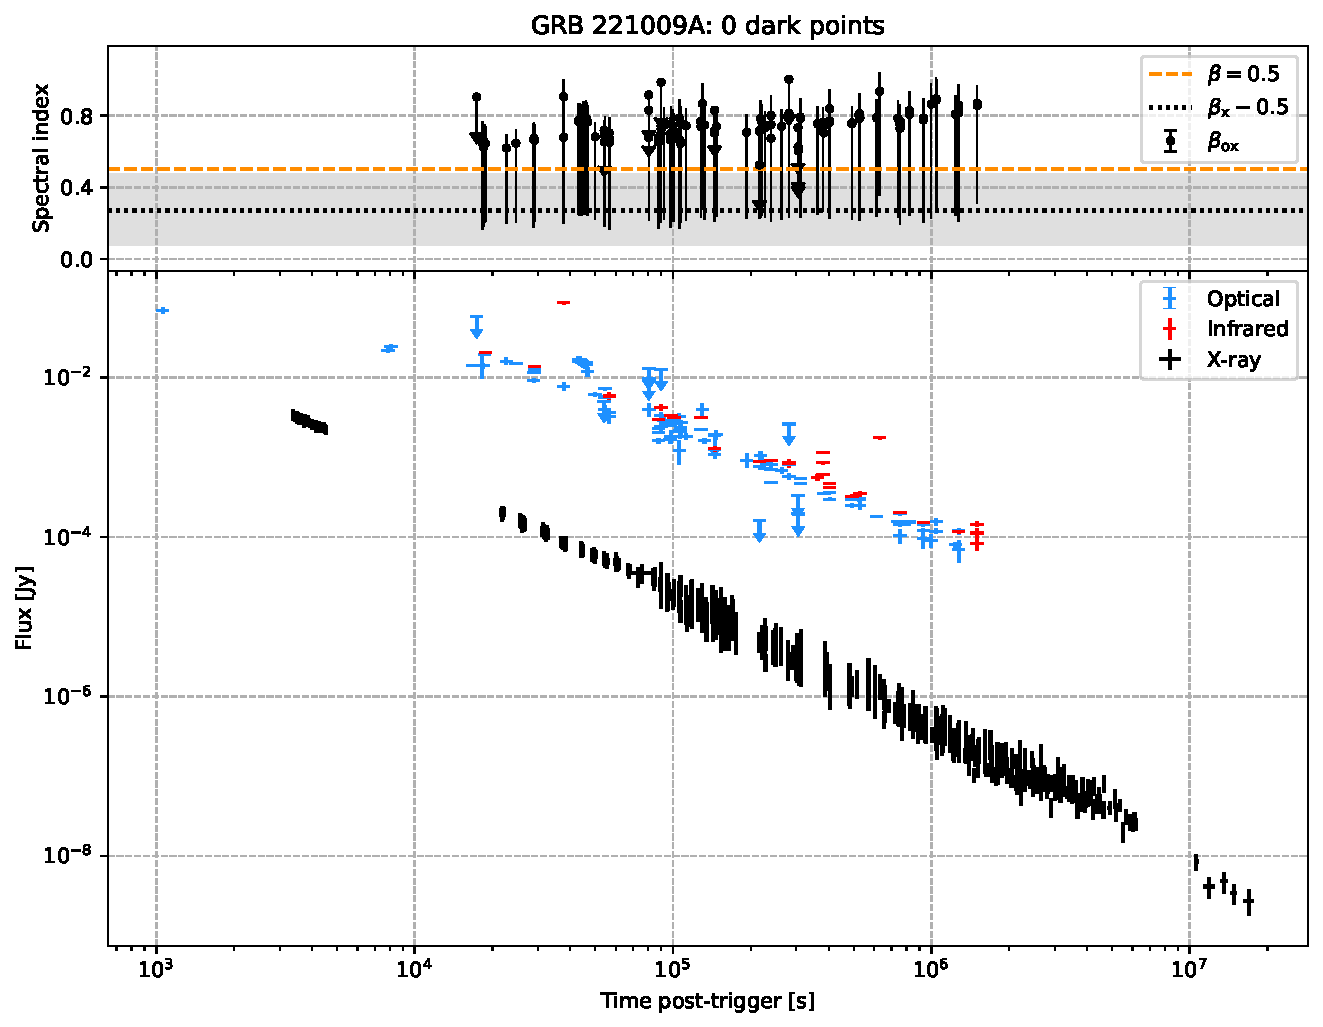
\includegraphics[width=0.80\linewidth]{appendix_figures/dark_lightcurves_221009A.pdf}
    \caption{Constructed light curve for GRB 221009A.}
    \label{221009A}
\end{figure}



\end{document}
